\chapter{Observation data \& Analysis
\label{chap:Orion-KL}}
\section{Observation data}
We analyzed 2 ALMA archival data. First, we used Cycle 2 data (ADS/JAO.ALMA\#2013.1.00553.S, 
\cite{Pagani+2017}) 
We also employed the ALMA Science Verification (SV) data (ADS/JAO.ALMA\#2011.0.00009.SV) 
at band 6 to fill up the missing frequency coverage of Cycle 2 data. 
\renewcommand{\arraystretch}{1.5}
\begin{table}[htb]
\begin{center}
  \caption{Summary of Observations}
  \label{tab:Obs_Ori}
{\scriptsize
  \begin{tabular}{lllllll} \hline \hline
 & Window & Frequency range & FWHM & PA \\
Date & (spw)  & (GHz) & (arcsec) & (degree) \\ \hline 
20 January 2012 (SV) & 0--16 & 213.715--246.627& 1.8$\times$1.3 & -1  \\  \hline
29--30 December 2014 (Cycle 2)&1 & 215.145--216.087 & 1.8 $\times$1.1 & 86 \\
&2 & 216.342--217.279 & 1.8 $\times$1.1 & 84 \\
&3 & 217.273--218.211 & 2.2 $\times$1.0 & 102 \\
&4 & 218.204--219.141 & 2.2 $\times$1.0 & 102 \\
&5 & 219.127--220.064 & 1.9 $\times$1.0 & 95 \\
&6 & 219.784--220.721 & 1.8 $\times$1.0  & 95 \\
&7 & 229.757--230.694 & 1.4 $\times$0.8 & 80 \\
&8 & 230.699--231.636 & 2.1 $\times$0.9 & 102 \\
&9 & 232.238--233.175 & 1.6 $\times$1.0 & 80 \\
&10 & 233.470--234.422 & 1.6 $\times$0.8 & 90 \\
&11 & 235.084--236.021 & 1.7 $\times$0.9 & 95 \\
&12 & 236.267--237.206 & 1.6 $\times$0.9 & 87 \\
&13 & 244.834--245.771 & 1.6 $\times$0.9 & 79 \\
&14 & 245.773--246.710 & 1.6 $\times$0.9 & 79 \\
&15 & 250.154--251.091 & 1.5 $\times$0.9 & 88 \\
&16 & 251.079--252.016 & 1.3 $\times$0.8 & 86 \\ \hline
  \end{tabular}
  }
\end{center}
\end{table}
Details of each data are summarized in Table \ref{tab:Obs_Ori}.

Cycle 2 data cube was already calibrated by Pagani et al., and the reduced data are available on 
the web site of CDS (Centre de Donnees astronomiques de Strasbourg)\footnote{http://cdsarc.u-strasbg.fr/viz-bin/qcat?J/A+A/604/A32}.
Since the SV data contained not only line emission but continuum emission, 
we subtracted continuum emission statistically by the method described in Section \ref{sec:Statcont}.

In addition, we used Common Astronomy Software Applications (CASA) software V.5.0.0 \citep{McMullin+2007} during the procedure to analyze observational data.

\newpage
\section{Analysis}
\subsection{Reduction of SV data}
\label{sec:Statcont}

With the advent of highly sensitive facilities such as ALMA, the spectral lines which were hindered 
by the noise level with the previous telescope can now be detected.
Most of these line-rich sources including hot cores are associated with detectable continuum emission.
In the analysis of molecular emission lines, the determination and the subtraction of this continuum 
emission is an essential, but difficult task. 
Therefore, we improved the method devised in \citet{Sanchez-Monge+2017} and deduced continuum subtraction 
in the observed $(u,v)$ domain (the raw visibilities measured by the interferometer).
We introduce the method and results in this section.

\subsubsection*{Determination of the continuum level}
The determination of the continuum emission level of astronomical sources observed in a spectral line 
observing mode is based on the identification of channels free of line emission, i.e. line-free channels.

First, we obtain the spectra for which we want to estimate the continuum level.  
In the case of Orion-KL, many molecular emission exist in Hot core
(RA$_{J2000}: 05^{\rm{h}}35^{\rm{m}}14^{\rm{s}}.580$, Dec$_{J2000}:-05^{\circ}22'31''.029$) or 
Compact ridge (RA$_{J2000}: 05^{\rm{h}}35^{\rm{m}}14^{\rm{s}}.2775$, Dec$_{J2000}:-05^{\circ}22'30''.776$), 
so we extracted spectra from circular regions with a diameter of 1''.0  with the coordinates indicated by 
\citet{Hirota+2015} as the center.
The peak of the distribution of the intensity values is determined with a Gaussian fit 
by assuming the Gaussian random error distribution with the mean value $E$ and the standard deviation $\sigma$.
The width is small in case of pixels with little or no line emission, but for line contaminated 
regions the distribution becomes broader and the exact location of the peak more uncertain. 
Therefore, we set the range of the Gaussian fitting from 0 to 1/3 of the peak intensity in line contaminated side 
and calculated the mean value $E$ and the standard deviation $\sigma$ (see Figure 2.1). 

\begin{figure}[hbp] 
\centering
\vspace{-0.5cm}
\includegraphics[width=0.7\textwidth]{OrionKL/ex_histogram_fit.eps}
\label{fig:histo}
\vspace{-1.5cm}
\caption{Schematic description of the process of determination of the continuum level toward Orion-KL: 
shown are the flux density distributions of Hot core (histogram) with the resulting fit overlaid (red line).}
\end{figure}

\newpage

\subsubsection*{Imaging line cubes}
Subsequently, the part of the distribution within $E - 3\sigma$ is defined as line-free channels.
Hot core and Compact ridges have different spectra because of the disparate chemical composition, 
so we determined the line-free channels individually and subtracted the continuum
in the $(u,v)$ domain by CASA task {\sc uvcontsub} with channels common to the two regions.
After the continuum subtraction, CASA task {\sc clean} was used to deconvolve the images by applying natural weighting.
The synthesized beam size of each data cube is listed in Table \ref{tab:Obs_Ori}. 
The velocity resolution is 0.6 km s$^{-1}$ for Cycle 2 data and 0.7 km s$^{-1}$ for SV data respectively.

Figure \ref{SVspec} shows examples of original and continuum-subtracted spectra towards Hot core. 
Since the baseline defined in this analysis seems to be reasonable, the continuum subtraction has succeeded.

\begin{figure}[htbp]
  \centering
  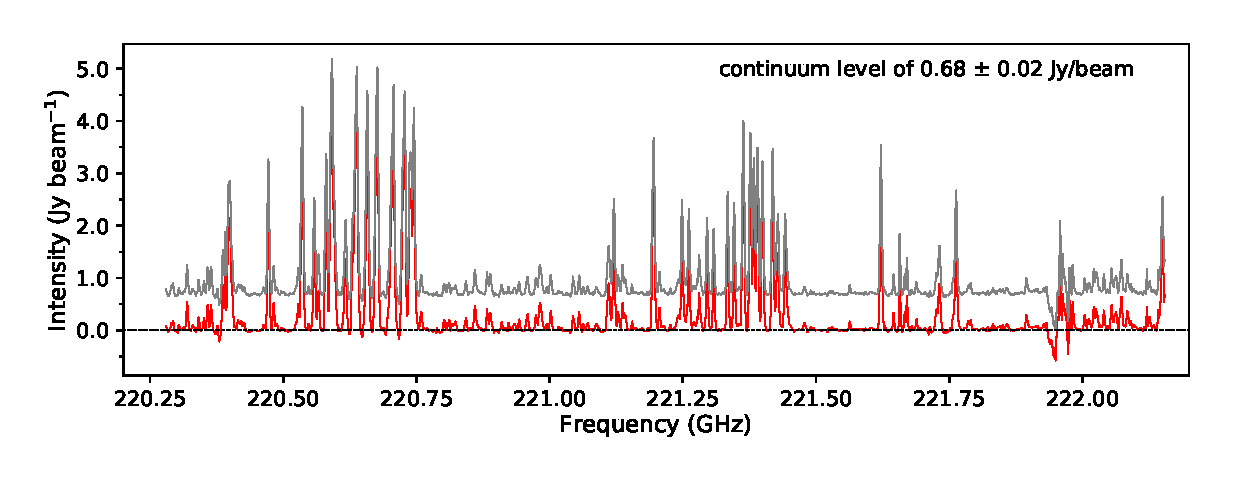
\includegraphics[width=0.98\textwidth]{OrionKL/spec_spw2.eps}
  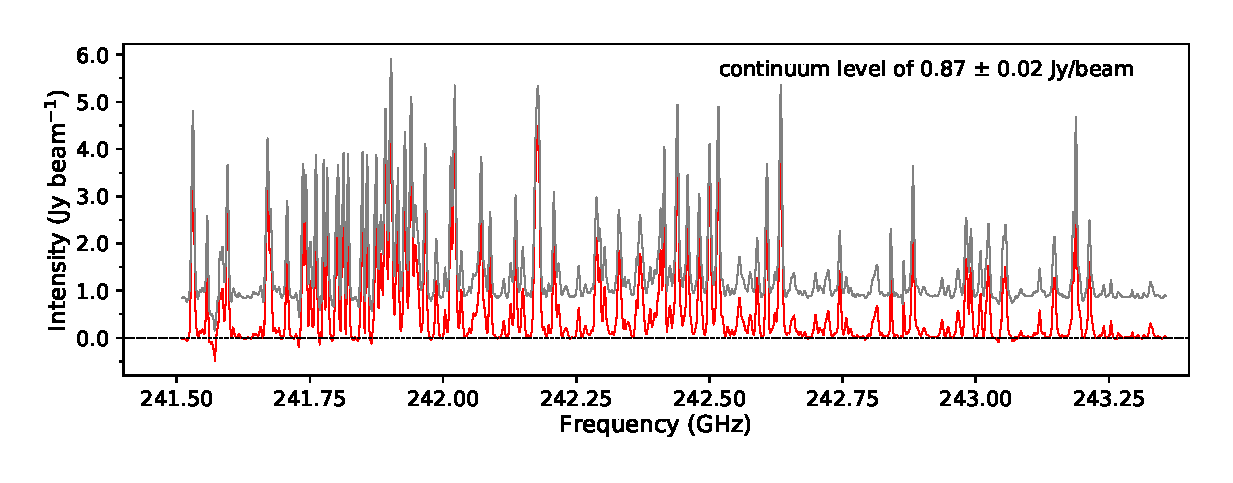
\includegraphics[width=0.98\textwidth]{OrionKL/spec_spw13.eps}
  \caption{The original spectra (gray) and continuum-subtracted spectra (red) towards Hot core. 
  The dotted line represents the base line (0 level). The continuum emission level subtracted from the original spectra, 
  together with its uncertainty, is listed in the upper right part of each panel.}
  \label{SVspec}
\end{figure}


\newpage
\subsection{Line identification}
Line selection and identification were carried out according to the following procedure.

\begin{enumerate}
\item The transition lines of CH$_3$NH$_2$ contained within the frequency coverage of the observation data were listed from the catalog. Spectroscopic data of CH$_3$NH$_2$ are provided by \citet{Motiyenko+2014} and JPL Molecular Spectroscopy catalog\footnote{http://spec.jpl.nasa.gov}.
We considered that detection of high excitation temperature or weak line strength transition 
is not realistic, and set thresholds that $S\mu^2 > 25\,\mathrm{D^2}$ and $E_{\mathrm{u}} < 200 \,\mathrm{K}$. We note that line strength $S$, the dipole moment $\mu$, and the upper state energy 
$E_{\mathrm{u}}$. Intensity is proportional to $S\mu^2$.

In addition, using the catalog obtained from JPL database, the Cologne database for molecular 
spectroscopy (CDMS)\footnote{https://cdms.ph1.uni-koeln.de/cdms/portal/}, 
and Splatalogue\footnote{http://www.splalogue.net/}'s "Hot Cores" filter, 
we investigated transitions of other species possibly contaminated within $\pm$2 km~s$^{-1}$  
around the rest frequency of CH$_3$NH$_2$. 
If other molecular emission lines exist with an offset of 2 km~s$^{-1}$ or larger, they are expected to spectrally resolve with high-velocity resolution (0.7 km s$^{-1}$ for SV data, 0.6 km s$^{-1}$ for Cycle 2).
Because it was hard to distinguish from CH$_3$NH$_2$, transitions with such contamination were excluded from the analysis.

The selection criteria of other species were set as follows; 
the transitions whose $E_{\mathrm{u}}$ is lower than $500\, \mathrm{K}$.
Transitions of CH$_3$NH$_2$ which is predicted to be blended were excluded from the survey.

As a result of the catalog selection, 24 transitions were listed from 201 transitions as detection candidates.

\item In order to find regions where signals exist in common among a series of data sets, 
we drew integrated intensity maps 
using CASA task {\sc immoment}. The integrated velocity range is 3.0-12.0 km s$^{-1}$, corresponding to
the typical velocity component of Hot core (4.8-6 km s$^{-1}$) and that of Compact ridge 
(7.2-9.6~km~s$^{-1}$). These values were adopted from \citet{Feng+2015}.

\item Emission at the center of Hot core was found in most of the integrated intensity maps. 

\item We extracted spectrum for transitions with no line blending around $\pm$2 km~s$^{-1}$ from Hot core. Here we checked again for blending. We investigated whether wider features existed 
in the spectrum subtracted from Hot core by eye and selected 6 lines among 24 transitions.

\item Subsequently, we estimated the systemic velocity and the line width of CH$_3$NH$_2$ 
by the Gaussian fitting from 6~transitions (see Section 3.2, Table \ref{tab:paraOri}).
\end{enumerate}
